\chapter{Evaluation and Testing}
\section{Introduction}
This section will review the work undertaken in chapter 3: Methodology. Chapter 3 broke the work flow down to 5 main headings, here 3 headings are discussed in relation to the outcome of the processes.

\section{Results of Clustering}
Fig.4.1. displays the graphical output from the clustering process. We clustered the time series consumption data based on mean consumption and based on the distribution of the mean energy consumption per half-hour per smart meter as seen in fig.3.3. we expected to see 3 clusters corresponding to low, medium and high consumption consumers of different sizes, for this reason we chose the max clusters to be 3. Fig.4.1. shows 3 distinct clusters highlighted in green, red and light blue. We can also observe that the green cluster is comparatively much larger than the other two clusters, based on number of observations contained within. The light blue and red clusters are relatively similar sizes with the red cluster being the smallest.

\begin{figure}
\centering     
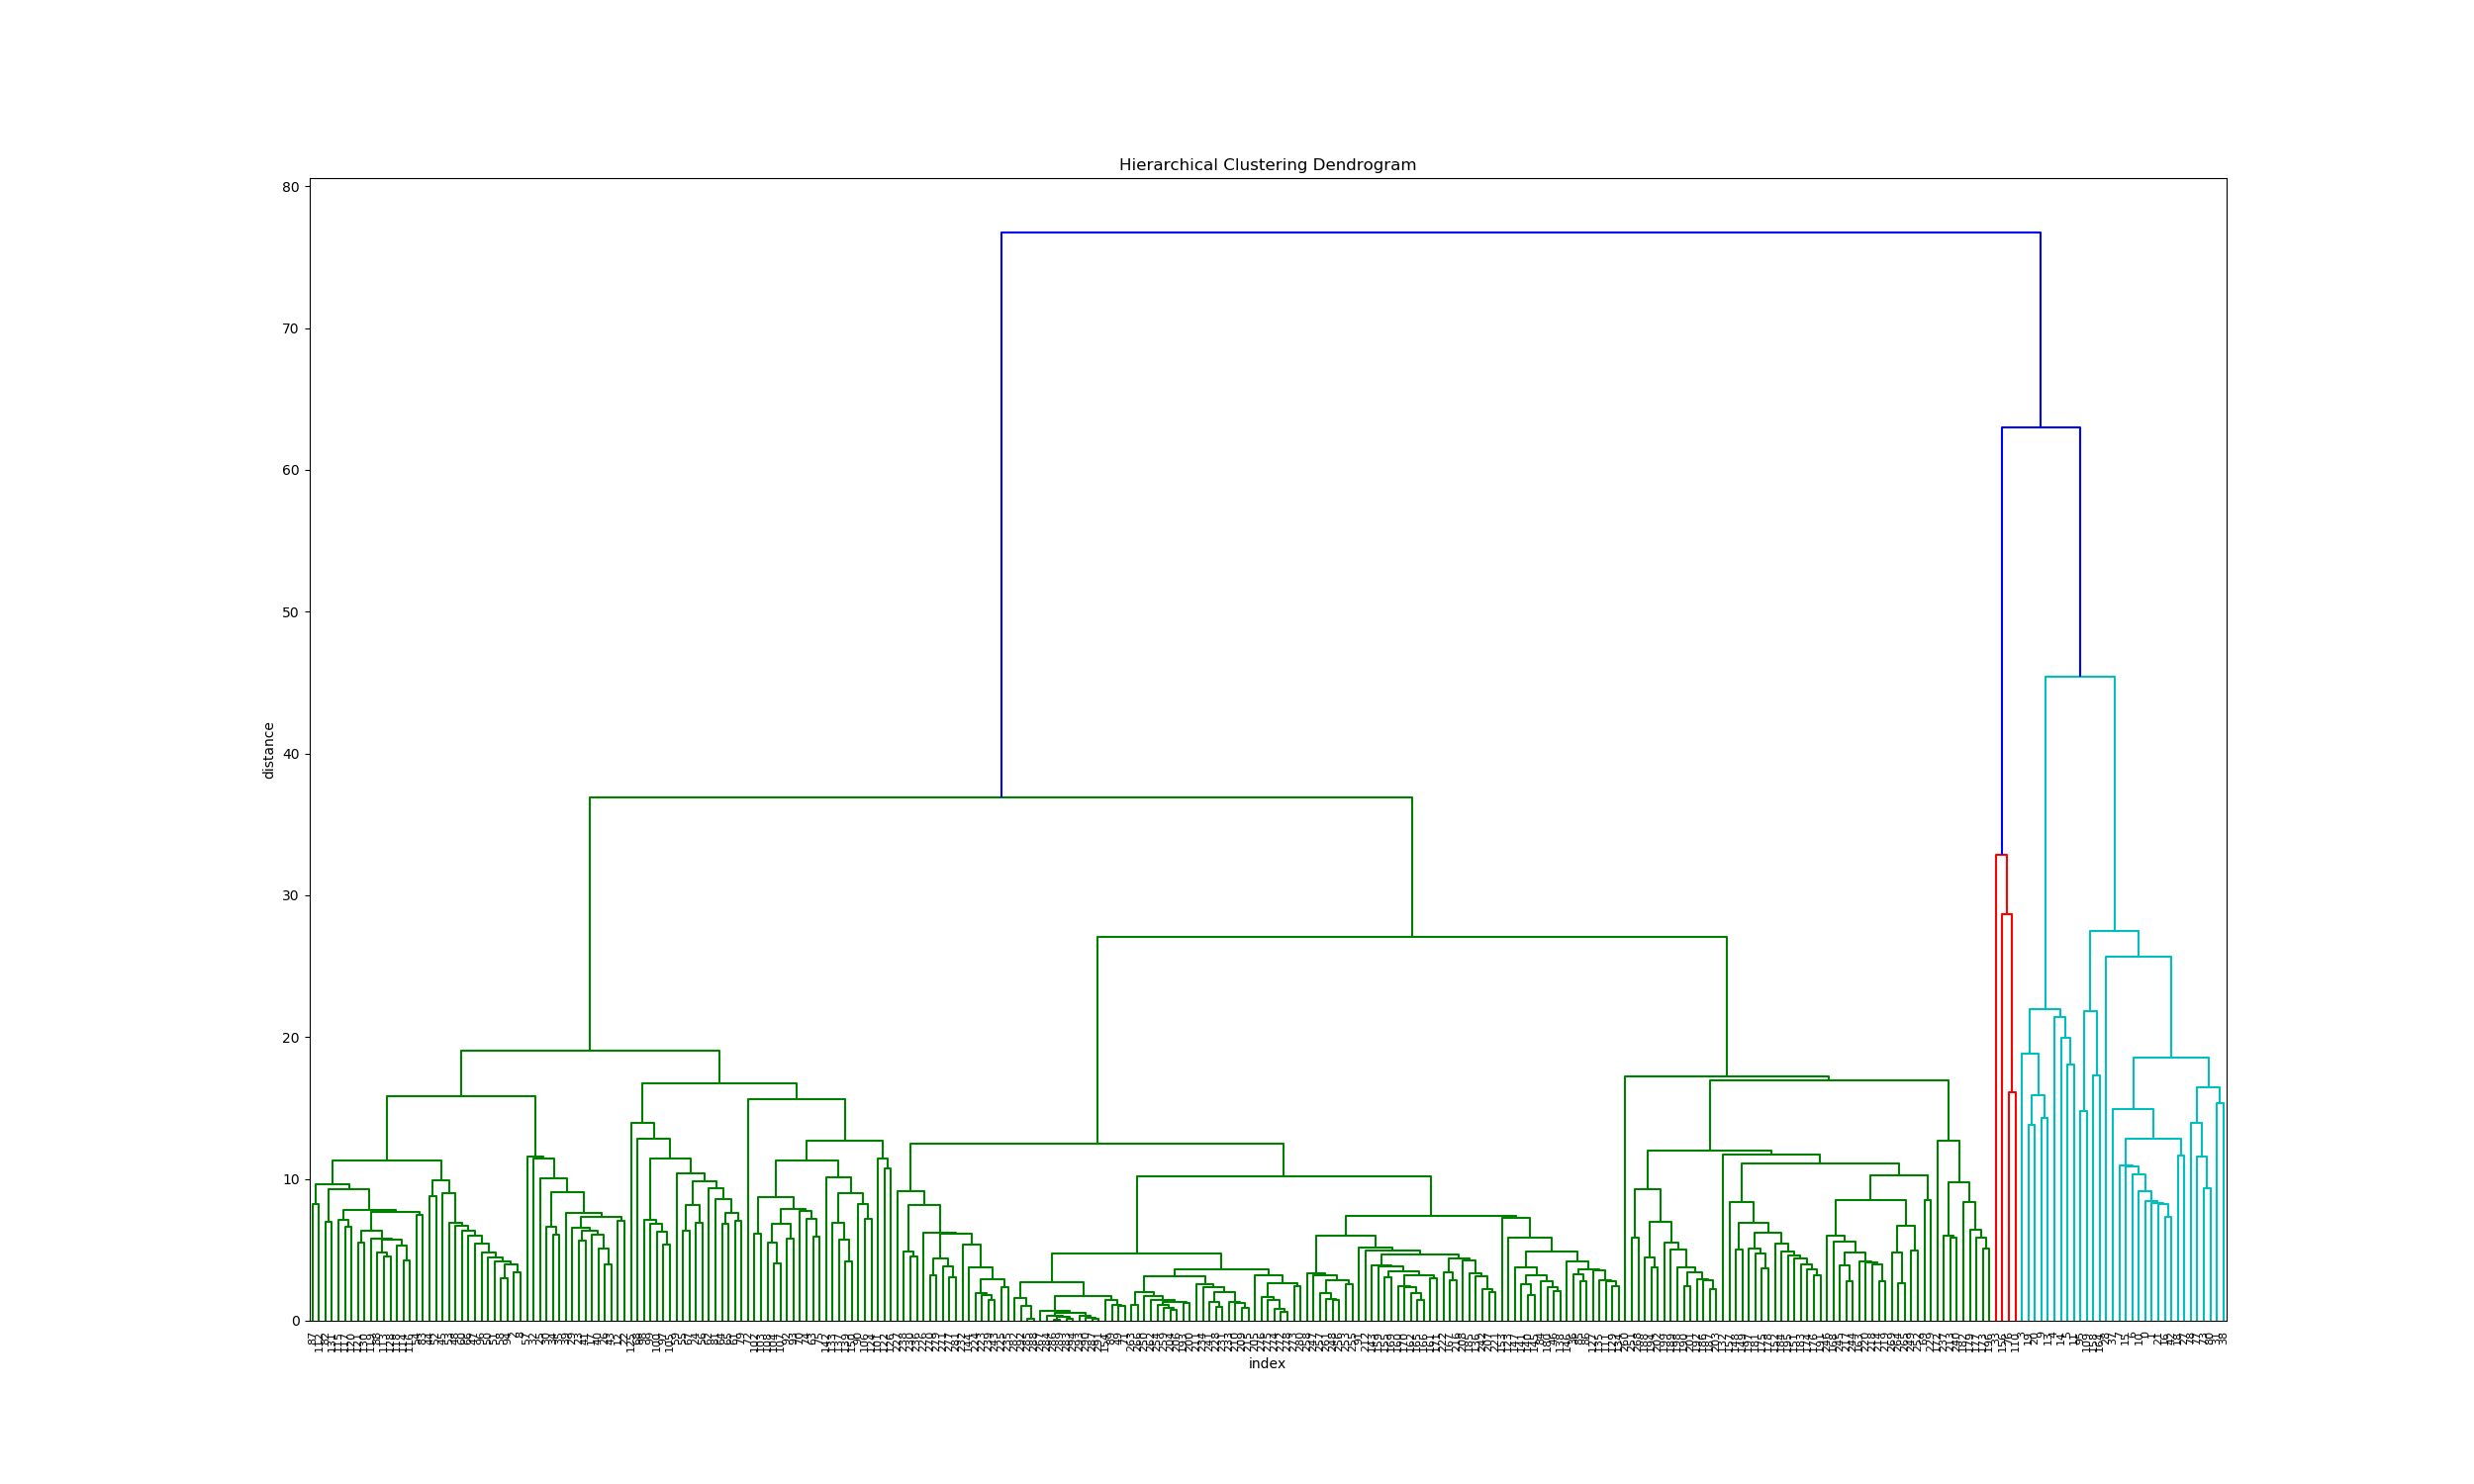
\includegraphics[width=1.7\textwidth, angle=90]{Figures/results/diagram.png}
\caption{Dendogram Generated from results of Hierarchical Clustering}
\label{fig:Dendrogram}
\end{figure} 

\subsection{Analysis of Clustering Results}
Each ANON\_ID in the data set was assigned a \textit{cluster\_id} based on the results of the hierarchical clustering, the time series data set can then be summarized with respect to each \textit{cluster\_id}.

\begin{figure}[H]
\centering     
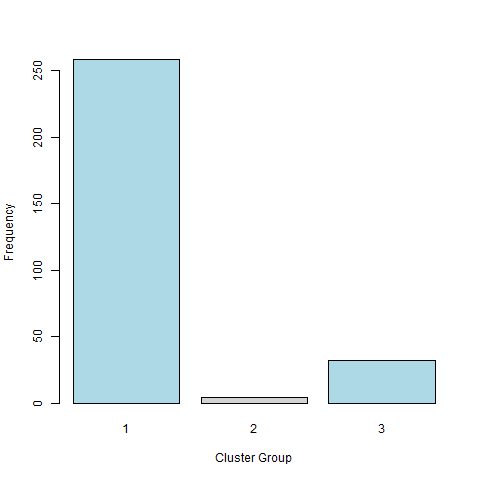
\includegraphics[width=1\textwidth]{Figures/results/cluster_bar.png}
\caption{Frequency of Cluster Groups}
\label{fig:Dendrogram}
\end{figure} 

Fig.4.2. shows the frequency of the cluster groups generated from the first chunk of data. It shows a class imbalance with the majority of the ANON\_IDs falling into the first cluster group.

\begin{figure}[H]
\centering     
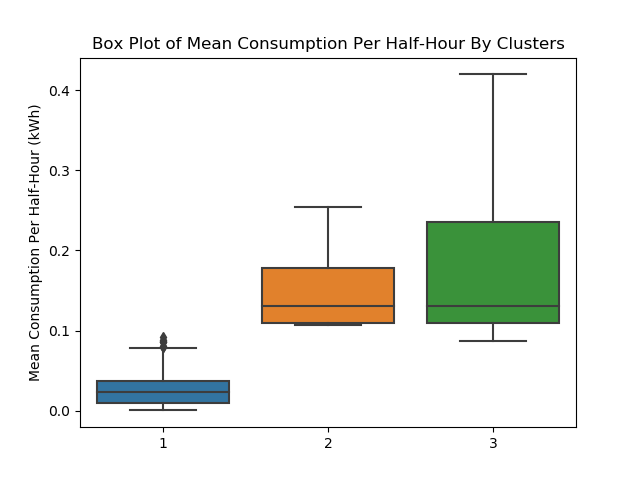
\includegraphics[width=1\textwidth]{Figures/results/clusters_boxplot.png}
\caption{Frequency of Cluster Groups}
\label{fig:Dendrogram}
\end{figure} 

In fig.4.3. we see the box plots representing the mean consumption per half-hour period of each cluster. As we can see the cluster 1 has the lowest mean with 0.02743 kWh, this cluster represents low energy consumption, low variation consumers. Clusters 2 \& 3 have very similar means with 0.15603 and 0.17238 kWh means respectively. These clusters represent high energy consumption with medium to high levels of variation. One factor separating the clusters 2 and 3 is the variation, we can see that cluster 3 has a much wider \textif{IQR} and the top whisker itself extends far above any value in the second cluster.


\section{Results of Random Forest Model}
In this section, the performance of the random forest model built will be evaluated with reference various graphs generated. Included is 2 other models, Gradient Boosting (GBM) model and a Support Vector Machine(SVM) model, these are included for comparison.

\begin{figure}[H]
\centering     
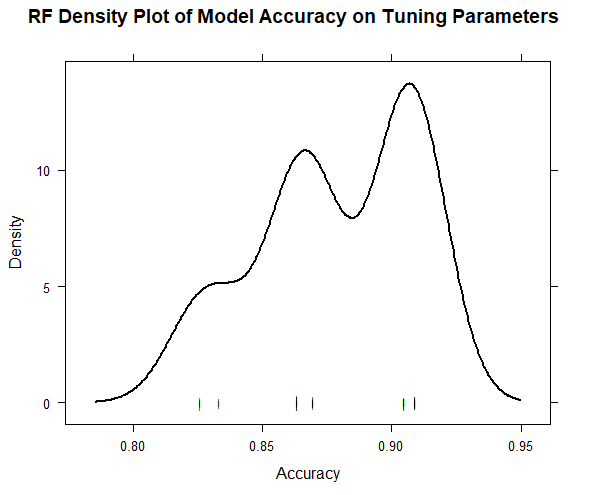
\includegraphics[width=0.7\textwidth]{Figures/results/rf_density.png}
\caption{RF density}
\label{fig:Dendrogram}
\end{figure} 

\begin{figure}[H]
\centering     
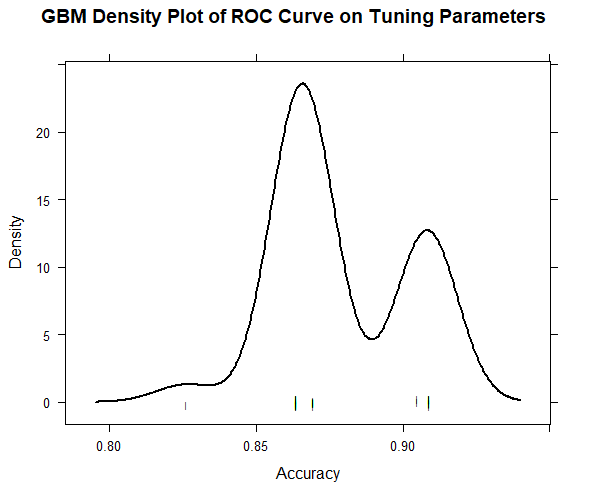
\includegraphics[width=0.7\textwidth]{Figures/results/gbm_density.png}
\caption{GBM density}
\label{fig:Dendrogram}
\end{figure} 

\begin{figure}[H]
\centering     
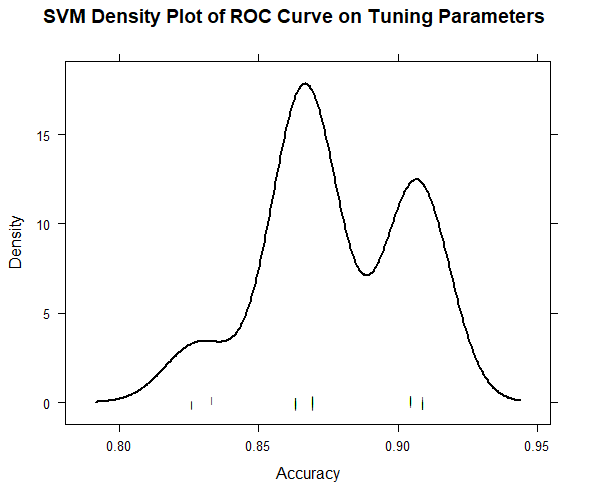
\includegraphics[width=0.7\textwidth]{Figures/results/svm_density.png}
\caption{SVM Density}
\label{fig:Dendrogram}
\end{figure} 

\textbf{Fig.4.4:4.6} shows the density plot of a given models accuracy based on the tuning parameters over a 10-fold Cross Validation (CV), repeated 10 times. All models show that depending on the tuning parameters, the accuracy was found to typically fall between 0.85 and 0.9. However this is misleading, fig.4.2. shows the frequency of the cluster groups in the chunk of data. This shows that there is an imbalance of clusters, 259, 4 and 32 observations belonging to cluster groups 1, 2 and 3 respectively.

\begin{figure}[H]
\centering     
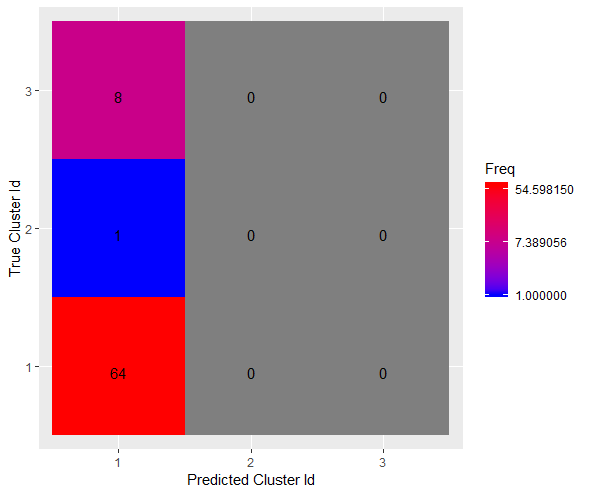
\includegraphics[width=0.8\textwidth]{Figures/results/confusion_matrix.png}
\caption{Confusion Matrix For Predicted Test Set}
\label{fig:Dendrogram}
\end{figure} 

\textbf{Fig.4.7.} shows the confusion matrix output, it compares the predicted cluster ids using the RF model built vs actual cluster they belonged to (according to our clustering model). The x-axis represents the cluster id the RF model assigned an ANON\_ID from the test set, this is the predicted label. The y-axis represents the cluster id assigned to a ANON\_ID from the clustering process, this is true label. In this figure we can see that there are a total of 73 observations in the test set. 64 belong to cluster id 1, 1 to cluster id 2 and 8 to cluster id 3. We can also see that our model predicted all of the observations to belong to cluster 1.